\documentclass{article}
\usepackage[utf8]{inputenc}
\usepackage{amsmath}
\usepackage{graphicx}
%\usepackage{enumerate}
\usepackage{amsfonts}
\usepackage{natbib}
\usepackage{url} % not crucial - just used below for the URL 
\usepackage{cleveref}
\usepackage{float}
\usepackage{subfigure}
%\usepackage{lineno,hyperref} 
\usepackage{xcolor}

%\pdfminorversion=4
% NOTE: To produce blinded version, replace "0" with "1" below.
\newcommand{\blind}{0}
\let\oldref\ref
\renewcommand{\ref}[1]{(\oldref{#1})}
\DeclareMathOperator*{\argmin}{argmin}
\DeclareMathOperator*{\argmax}{argmax}


\newtheorem{prop}{Proposition}
\newtheorem{assumption}{Assumption}
\newtheorem{thm}{Theorem}
\newtheorem{proof}{Proof}


\title{Simulation and Timeline}
%author{xmengju }
%\date{March 2021}

\begin{document}
\maketitle


\section{Robust TFBoost: Simulation}
\subsection{Data generation}
\begin{itemize}
    \item We generated data sets $D = \{(x_i, y_i), i = 1,..., N\}$, consisting of a predictor $x_i\in\mathcal{L}_2$ and a scalar response $y_i$ that follow the model: 
 \begin{equation} \label{eq:gen}
y_i = r(x_i) + \rho \epsilon_i,
\end{equation}
where the errors $\epsilon_i$ are i.i.d, $r$ is the regression function,  and  $\rho > 0$ is a constant that controls the signal-to-noise ratio (SNR): 
$$\text{SNR} = \frac{\text{Var}(r(X))}{\text{Var}(\rho\epsilon)}.$$
\item To sample the functional predictors $x_i$, we considered the model:

\begin{equation} \label{eq:xmodel}
    x_i(t) = \mu(t) + \sum_{p=1}^4 \sqrt{\lambda_j}\xi_{ij}\phi_j(t),
\end{equation}
where $\mu(t) = 2\text{sin}(t\pi) \text{exp}(1-t)$, $\lambda_1 = 0.8, \lambda_2 = 0.3, \lambda_3 = 0.2$, and $\lambda_4 = 0.1$,  $\xi_{ij}\sim N(0,1) $,  and $\phi_j$ are the first four eigenfunctions of the ``Mattern'' covariance function $\gamma(s,t)$ with parameters $\rho = 3, \sigma = 1, \nu = 1/3$: 
 $$\gamma(s,t) = C\left(\frac{\sqrt{2\nu}|s-t|}{\rho}\right), \ C(u) = \frac{\sigma^2 2^{1-\nu}}{\Gamma(\nu)} u^{\nu} K_{\nu}(u),$$
  where $\Gamma(.)$ is the Gamma function and $K_{\nu}$ is the modified Bessel function of the second kind. For each subject $i$, we evaluate $x_i$ on a dense and regular grid $t_1,..., t_{100}$ equally spaced in $\mathcal{I} = [0,1]$. 
\item We considered five regression functions:
\begin{itemize}

\item[- ]  $r_1(X) =  \int_{\mathcal{I}} \left (\text{sin} \left(\frac{3}{2} \pi t \right) +  \text{sin} \left(\frac{1}{2} \pi t \right)\right)X(t)dt,$
\item[- ]  $r_2(X) = (\xi_1 + \xi_2)^{1/3},$ where  $\xi_1 = \int_{\mathcal{I}} (X(t) - \mu(t))\psi_1(t) dt$ and $\xi_2 = \int_{\mathcal{I}} (X(t) - \mu(t))\psi_2(t) dt$ are projections onto the first two FPCs ($\psi_1$ and $\psi_2$) of $X$ with mean $\mu(t) = E(X(t))$, 
\item[- ]  $r_3(X) = 5\text{exp}\left (- \frac{1}{2}\left| \int_{\mathcal{I}} x(t)\log(|x(t)|)dt \right| \right),$
\item[- ] 
$r_4(X) = 5\text{sigmoid}\left(\int_{\mathcal{I}}X(t)^2 \text{sin}(2\pi t) dt \right),$ where  $\text{sigmoid}(u) = 1/(1+ \text{exp}(-u))$, and
\item[- ] 
$r_5(X) = 5 \left( \sqrt{\left|\int_{\mathcal{I}_1} \text{cos}(2\pi t^2) X(t) dt \right|} + \sqrt{\left|\int_{\mathcal{I}_2} \text{sin}(X(t)) dt \right|} \right), $ where  $\mathcal{I}_1 = [0,0.5]$ and $\mathcal{I}_2 = (0.5,1]$. 
\end{itemize}

\item For clean data ($C_0$), we generated $\epsilon_i$ in \ref{eq:gen} from $N(0,1)$ and selected $\rho$ that corresponds to SNR = 5. 

For contaminated data, we sampled 10\% training samples as outliers and let the set of their indices be $I_{\text{o}}$. The outliers belong to  one of the five types introduced below. For $j \in I_{\text{o}}$, 
\begin{itemize}
    \item[- ] $C_1$: \textit{Shape outliers}
    
    \vspace{1ex}
    In \ref{eq:gen}, $\epsilon_j \sim N(10, 0.25)$ \\
    In \ref{eq:xmodel},   $\xi_{j,2} \sim N(10, 0.25)$ and the other parameters stay the same.  
       \vspace{1ex}
    \item[- ] $C_2$: \textit{Magnitude outliers}     \vspace{1ex}
    
    $x_{j} = 2 \tilde{x}_{j}, y_{j} =  4 \tilde{y}_{j},$ where $(\tilde{x}_j, \tilde{y}_j)$ were generated as clean data.
       \vspace{1ex}
    \item[- ] $C_3$: \textit{Point-type measurement error outliers} 
    
       \vspace{1ex}
   Randomly sample 10  points form $t_1,..., t_{100}$ and denote them as $t_{j,o_1},..., t_{j,o_{10}}$. For $k = 1,..., 10$,   
    $$x_{j}(t_{j,o_k}) = \tilde{x}_j(t_{j,o_k}) + \eta_{j,o_k},$$ where $\eta_{j,o_k} \sim 0.5 N(10, 0.25) + 0.5 N(-10, 0.25)$, $y_j = \tilde{y}_j$, and 
 $(\tilde{x}_j, \tilde{y}_j)$ were generated as clean data. 
    \vspace{1ex}
    \item[- ] $C_4$: \textit{Interval-type measurement error outliers} 
    
       \vspace{1ex}
     Randomly sample one interval from intervals $[t_1,...,t_{10}]$, ...,$[t_{91},...,t_{100}]$,   and denote the interval as $t_{j,o},..., t_{j,o+9}$
     
     For $k = 0,..., 9$,   
    $$x_{j}(t_{j,o + k}) = \tilde{x}_j(t_{j,o + k}) + \eta_{j,o+k},$$ where $\eta_{j,o + k} \sim  N(10, 0.25)$, $y_j = \tilde{y}_j$, and 
 $(\tilde{x}_j, \tilde{y}_j)$ were generated as clean data. 
    \vspace{1ex}
 
    \item[- ] $C_5$: \textit{Pure vertical outliers} 
       \vspace{1ex}
   $$\epsilon_{j} \sim N(10, 0.25)$$
\end{itemize}
\end{itemize}


\subsection{Visualize the outliers}

\begin{figure}[H]
    \centering
    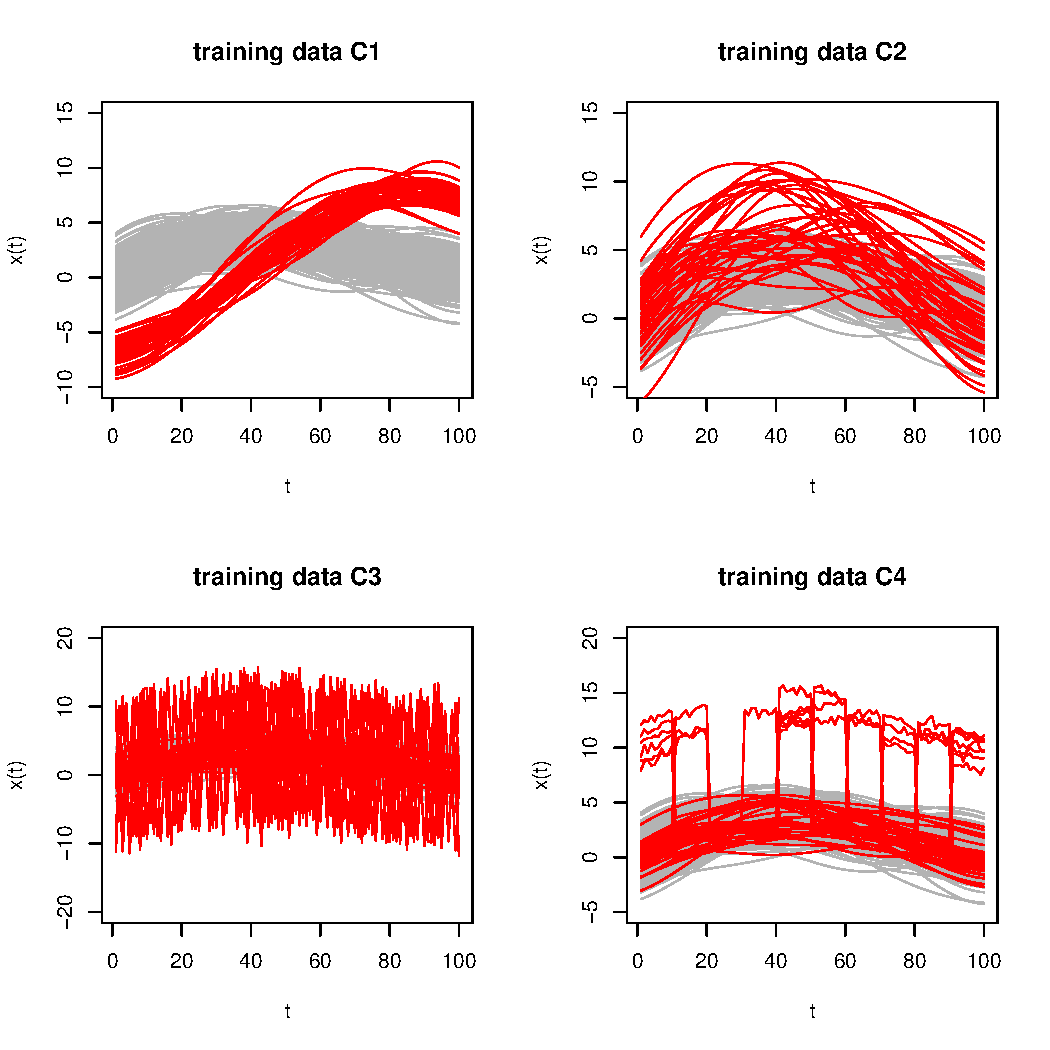
\includegraphics[scale = 0.8]{visualize_outliers.pdf}
\end{figure}

\subsection{Model comparison}
For each setting, we used 100 independently generated datasets and compared the performance of the following methods: 

\begin{itemize}
 \setlength\itemsep{0.1em}
\item  \texttt{TFBoost(L2)}:  tree-based functional boosting with L2 loss
\item  \texttt{TFBoost(LAD)}:  tree-based functional boosting with LAD loss
\item  \texttt{TFBoost(RR)}:  tree-based functional boosting modified to follow the framework of RRBoost
\item \texttt{FPPR}: functional projection pursuit regression \citep{ferraty2013functional},
\item \texttt{FGAM}: functional generalized additive models \citep{mclean2014functional}, 
\item \texttt{MFLM}: Sieve M-estimator for a semi-functional linear model \cite{huang2015sieve}
\item \texttt{RFSIR}: robust functional sliced inverse regression \citep{wang2017robust}
\item \texttt{RFPLM}: robust estimation for semi-functional linear regression models \citep{boente2020robust}
\end{itemize}

\subsection{Results}
% latex table generated in R 4.0.5 by xtable 1.8-4 package
% Mon Aug  2 23:50:53 2021
\renewcommand{\arraystretch}{1.5}
\addtolength{\tabcolsep}{-3pt}    
\begin{table}[H]
\footnotesize
\centering
\begin{tabular}{rllllll}
  \hline
 & $C_0$ & $C_1$ & $C_2$ & $C_3$ & $C_4$ & $C_5$ \\ 
  \hline
TFBoost(L2) & 0.146 (0.005) & 0.604 (0.304) & 0.878 (0.275) & 0.991 (0.317) & 1.163 (0.333) & 1.294 (0.806) \\ 
  TFBoost(LAD) & 0.150 (0.009) & 0.197 (0.110) & 0.194 (0.070) & 0.147 (0.014) & 0.250 (0.195) & 0.153 (0.010) \\ 
  TFBoostLAD-M) & 0.148 (0.009) & 0.285 (0.173) & 0.222 (0.069) & 0.172 (0.026) & 0.486 (0.372) & 0.152 (0.011) \\ 
  TFBoost(RR) & 0.150 (0.010) & 0.804 (1.765) & 0.284 (0.391) & 0.268 (0.317) & 1.306 (2.452) & 0.150 (0.013) \\ 
  FPPR & 0.137 (0.006) & 3.378 (3.725) & 1.787 (2.510) & 6.025 (4.312) & 9.691 (6.253) & 2.759 (2.671) \\ 
  FGAM & \textbf{0.130} (0.005) & 1.751 (2.464) & 2.732 (3.324) & 62.725 (182.870) & 6.073 (15.833) & 0.848 (0.456) \\ 
  RFPLM & 0.131 (0.006) & \textbf{0.131} (0.006) & \textbf{0.131} (0.006) & \textbf{0.120} (0.001) & \textbf{0.130} (0.002) & \textbf{0.131} (0.006) \\ 
  MFLM & \textbf{0.130} (0.005) & \textbf{0.138} (0.009) & \textbf{0.181} (0.052) & \textbf{0.129} (0.016) & 0.168 (0.026) & \textbf{0.139} (0.011) \\ 
  RFSIR & 0.138 (0.007) & 0.465 (0.438) & 1.113 (0.932) & 0.130 (0.004) & \textbf{0.140} (0.006) & 1.207 (1.229) \\ 
   \hline
\end{tabular}
\caption{Summary statistics of test errors for data generated from $r_1$; displayed in the form of mean (sd).} 
\end{table}
% latex table generated in R 4.0.5 by xtable 1.8-4 package
% Mon Aug  2 23:51:08 2021
\begin{table}[H]
\footnotesize
\centering
\begin{tabular}{rllllll}
  \hline
 & $C_0$ & $C_1$ & $C_2$ & $C_3$ & $C_4$ & $C_5$ \\ 
  \hline
TFBoost(L2) & \textbf{0.183} (0.010) & 0.703 (0.369) & 1.013 (0.155) & 1.178 (0.285) & 1.468 (0.270) & 2.338 (1.533) \\ 
  TFBoost(LAD) & 0.186 (0.008) & \textbf{0.258} (0.167) & \textbf{0.251} (0.122) & 0.178 (0.008) & \textbf{0.254} (0.117) & \textbf{0.190} (0.014) \\ 
  TFBoostLAD-M) & 0.190 (0.008) & 0.333 (0.185) & 0.319 (0.266) & 0.224 (0.044) & 0.498 (0.251) & 0.195 (0.016) \\ 
  TFBoost(RR) & 0.192 (0.016) & \textbf{0.186} (0.011) & 0.848 (2.711) & \textbf{0.175} (0.013) & 0.404 (0.626) & \textbf{0.190} (0.017) \\ 
  FPPR & \textbf{0.182} (0.010) & 4.119 (3.694) & 3.156 (3.078) & 7.945 (6.784) & 9.384 (4.534) & 3.295 (2.602) \\ 
  FGAM & 0.226 (0.010) & 1.972 (2.451) & 2.941 (2.394) & 55.296 (163.996) & 6.197 (15.351) & 0.995 (0.475) \\ 
  RFPLM & 0.285 (0.012) & 0.283 (0.013) & \textbf{0.286} (0.013) & 0.274 (0.011) & 0.281 (0.014) & 0.286 (0.016) \\ 
  MFLM & 0.283 (0.011) & 0.358 (0.144) & 0.526 (0.197) & 0.567 (0.153) & 0.709 (0.056) & 0.477 (0.190) \\ 
  RFSIR & 0.184 (0.009) & 0.682 (0.636) & 1.647 (2.307) & \textbf{0.171} (0.005) & \textbf{0.199} (0.027) & 1.356 (1.319) \\ 
   \hline
\end{tabular}
\caption{Summary statistics of test errors for data generated from $r_2$; displayed in the form of mean (sd).} 
\end{table}
% latex table generated in R 4.0.5 by xtable 1.8-4 package
% Mon Aug  2 23:51:22 2021
\begin{table}[H]
\footnotesize
\centering
\begin{tabular}{rllllll}
  \hline
 & $C_0$ & $C_1$ & $C_2$ & $C_3$ & $C_4$ & $C_5$ \\ 
  \hline
TFBoost(L2) & \textbf{0.309} (0.013) & 0.956 (0.546) & 1.499 (0.360) & 1.668 (0.170) & 2.042 (0.248) & 2.414 (1.502) \\ 
  TFBoost(LAD) & 0.316 (0.016) & \textbf{0.391} (0.131) & \textbf{0.377} (0.090) & 0.301 (0.017) & 0.423 (0.203) & \textbf{0.324} (0.024) \\ 
  TFBoostLAD-M) & 0.317 (0.015) & 0.450 (0.130) & 0.395 (0.109) & 0.337 (0.043) & 0.641 (0.405) & 0.329 (0.023) \\ 
  TFBoost(RR) & 0.324 (0.032) & 0.710 (1.743) & 0.469 (0.477) & \textbf{0.290} (0.011) & \textbf{0.313} (0.021) & \textbf{0.315} (0.020) \\ 
  FPPR & \textbf{0.305} (0.019) & 3.352 (3.087) & 2.699 (3.097) & 6.614 (6.942) & 8.806 (4.622) & 2.996 (2.215) \\ 
  FGAM & 0.321 (0.017) & 2.006 (2.452) & 3.825 (3.861) & 52.164 (147.124) & 6.453 (15.311) & 1.107 (0.459) \\ 
  RFPLM & 0.380 (0.018) & \textbf{0.383} (0.017) & \textbf{0.380} (0.019) & 0.363 (0.014) & 0.386 (0.025) & 0.380 (0.021) \\ 
  MFLM & 0.377 (0.018) & 0.394 (0.021) & 0.475 (0.082) & 0.415 (0.030) & 2.596 (0.186) & 0.404 (0.024) \\ 
  RFSIR & 0.313 (0.018) & 2.423 (3.818) & 1.758 (2.426) & \textbf{0.292} (0.026) & \textbf{0.310} (0.016) & 1.455 (0.940) \\ 
   \hline
\end{tabular}
\caption{Summary statistics of test errors for data generated from $r_3$; displayed in the form of mean (sd).} 
\end{table}
% latex table generated in R 4.0.5 by xtable 1.8-4 package
% Mon Aug  2 23:51:36 2021
\begin{table}[H]
\footnotesize
\centering
\begin{tabular}{rllllll}
  \hline
 & $C_0$ & $C_1$ & $C_2$ & $C_3$ & $C_4$ & $C_5$ \\ 
  \hline
TFBoost(L2) & \textbf{0.323} (0.015) & 0.884 (0.472) & 1.596 (0.382) & 1.941 (0.344) & 2.073 (0.247) & 2.514 (1.598) \\ 
  TFBoost(LAD) & 0.335 (0.014) & \textbf{0.401} (0.140) & \textbf{0.392} (0.070) & \textbf{0.317} (0.017) & 0.565 (0.328) & 0.351 (0.039) \\ 
  TFBoostLAD-M) & \textbf{0.333} (0.020) & \textbf{0.470} (0.167) & \textbf{0.432} (0.128) & 0.343 (0.026) & 0.728 (0.382) & \textbf{0.343} (0.034) \\ 
  TFBoost(RR) & 0.335 (0.025) & 0.879 (2.194) & 0.468 (0.417) & \textbf{0.313} (0.035) & 1.252 (2.085) & \textbf{0.340} (0.034) \\ 
  FPPR & 0.364 (0.030) & 3.899 (3.073) & 3.696 (3.489) & 7.516 (5.231) & 10.841 (5.110) & 4.360 (2.674) \\ 
  FGAM & 0.409 (0.020) & 2.031 (2.307) & 3.775 (3.793) & 44.480 (120.133) & 6.741 (16.325) & 1.511 (0.452) \\ 
  RFPLM & 0.542 (0.034) & 0.544 (0.037) & 0.546 (0.043) & 0.525 (0.028) & \textbf{0.552} (0.028) & 0.546 (0.040) \\ 
  MFLM & 0.537 (0.032) & 0.610 (0.149) & 0.709 (0.168) & 0.825 (0.141) & 1.024 (0.106) & 0.764 (0.165) \\ 
  RFSIR & 0.340 (0.018) & 1.447 (1.648) & 3.148 (3.282) & 0.328 (0.018) & \textbf{0.352} (0.019) & 1.803 (0.843) \\ 
   \hline
\end{tabular}
\caption{Summary statistics of test errors for data generated from $r_4$; displayed in the form of mean (sd).} 
\end{table}
% latex table generated in R 4.0.5 by xtable 1.8-4 package
% Mon Aug  2 23:51:52 2021
\begin{table}[H]
\footnotesize
\centering
\begin{tabular}{rllllll}
  \hline
 & $C_0$ & $C_1$ & $C_2$ & $C_3$ & $C_4$ & $C_5$ \\ 
  \hline
TFBoost(L2) & \textbf{0.586} (0.034) & 1.087 (0.429) & 2.274 (0.690) & 2.369 (0.300) & 2.625 (0.289) & 3.078 (1.355) \\ 
  TFBoost(LAD) & 0.617 (0.033) & \textbf{0.726} (0.216) & \textbf{0.705} (0.054) & 0.603 (0.031) & \textbf{0.698} (0.098) & 0.649 (0.054) \\ 
  TFBoostLAD-M) & 0.607 (0.035) & \textbf{0.743} (0.196) & \textbf{0.740} (0.145) & \textbf{0.583} (0.038) & 0.875 (0.228) & \textbf{0.619} (0.048) \\ 
  TFBoost(RR) & 0.643 (0.045) & 0.825 (0.990) & 1.107 (1.602) & \textbf{0.578} (0.048) & 1.176 (1.296) & \textbf{0.619} (0.049) \\ 
  FPPR & 0.607 (0.062) & 4.380 (3.473) & 3.035 (3.747) & 6.109 (4.047) & 9.940 (3.798) & 4.196 (3.162) \\ 
  FGAM & \textbf{0.606} (0.041) & 2.278 (2.458) & 5.049 (5.805) & 43.774 (117.297) & 7.048 (13.854) & 1.857 (0.516) \\ 
  RFPLM & 0.896 (0.048) & 0.871 (0.053) & 0.892 (0.052) & 0.849 (0.040) & 0.896 (0.046) & 0.888 (0.053) \\ 
  MFLM & 0.883 (0.040) & 0.891 (0.045) & 1.034 (0.166) & 0.944 (0.071) & 2.009 (0.817) & 0.932 (0.071) \\ 
  RFSIR & 0.680 (0.056) & 2.423 (2.383) & 2.211 (1.382) & 0.628 (0.038) & \textbf{0.638} (0.049) & 1.979 (0.973) \\ 
   \hline
\end{tabular}
\caption{Summary statistics of test errors for data generated from $r_5$; displayed in the form of mean (sd).} 
\end{table}



\subsection{Timeline}
\begin{itemize}
    \item 2021/07: 
    \begin{itemize}
        \item  TFBoost: revise paper (submit?)
        \item Robust TFBoost: simulation 
        \item  thesis: draft the background chapter 
    \end{itemize}
   \item  2021/08:  \begin{itemize}
   \item  TFBoost: submit paper and package
        \item   thesis: draft the background,  RRBoost and TFBoost chapters 
        \item  Robust TFBoost: simulation and real example
        \item record JSM presentation
    \end{itemize}
    \item  2021/09:
    \begin{itemize}
    \item thesis: draft Robust TFBoost chapter
    \item Sparse TFBoost: simulation 
    \end{itemize}
   \item  2021/09:
    \begin{itemize}
    \item thesis: draft robust TFBoost, Sparse TFBoost chapters 
    \item Sparse TFBoost: simulation and real example
    \end{itemize}
    \item  2021/10:
    \begin{itemize}
    \item thesis: draft Sparse TFBoost chapter, conclusion and future work
    \end{itemize}
\item  2021/11:
    \begin{itemize}
    \item thesis: first draft complete, start revising 
    \end{itemize}
\item  2021/12 (end of year):     
\begin{itemize}
    \item thesis: second draft 
    \end{itemize}
\item Before  2022/04:
\begin{itemize}
    \item thesis defence 
    \end{itemize}
\end{itemize}

\bibliographystyle{apalike}
\bibliography{reference}
\end{document}
